\newpage
\section{Introduction}
V2X, short for vehicle-to-everything, is a technology meant to make traffic safer by letting the car communicate with its surroundings, covering up some of the blind spots in the drivers spacial perception and understanding. There are different types of communications that can be implemented in real life situations such as V2I (vehicle to infrastructure), V2G (vehicle to grid), V2D (vehicle to device), V2V (vehicle to vehicle), V2P (vehicle to pedestrian), V2N (vehicle to network) and V2TT (vehicle to tram and train). In this project we will focus on a special case of V2I where a car is moving towards a crossing in a simulation environment. This case makes us detect and understand some risks and problems of real world situations (\textit{see figure 1}).

\begin{figure}[H]
    \centering
    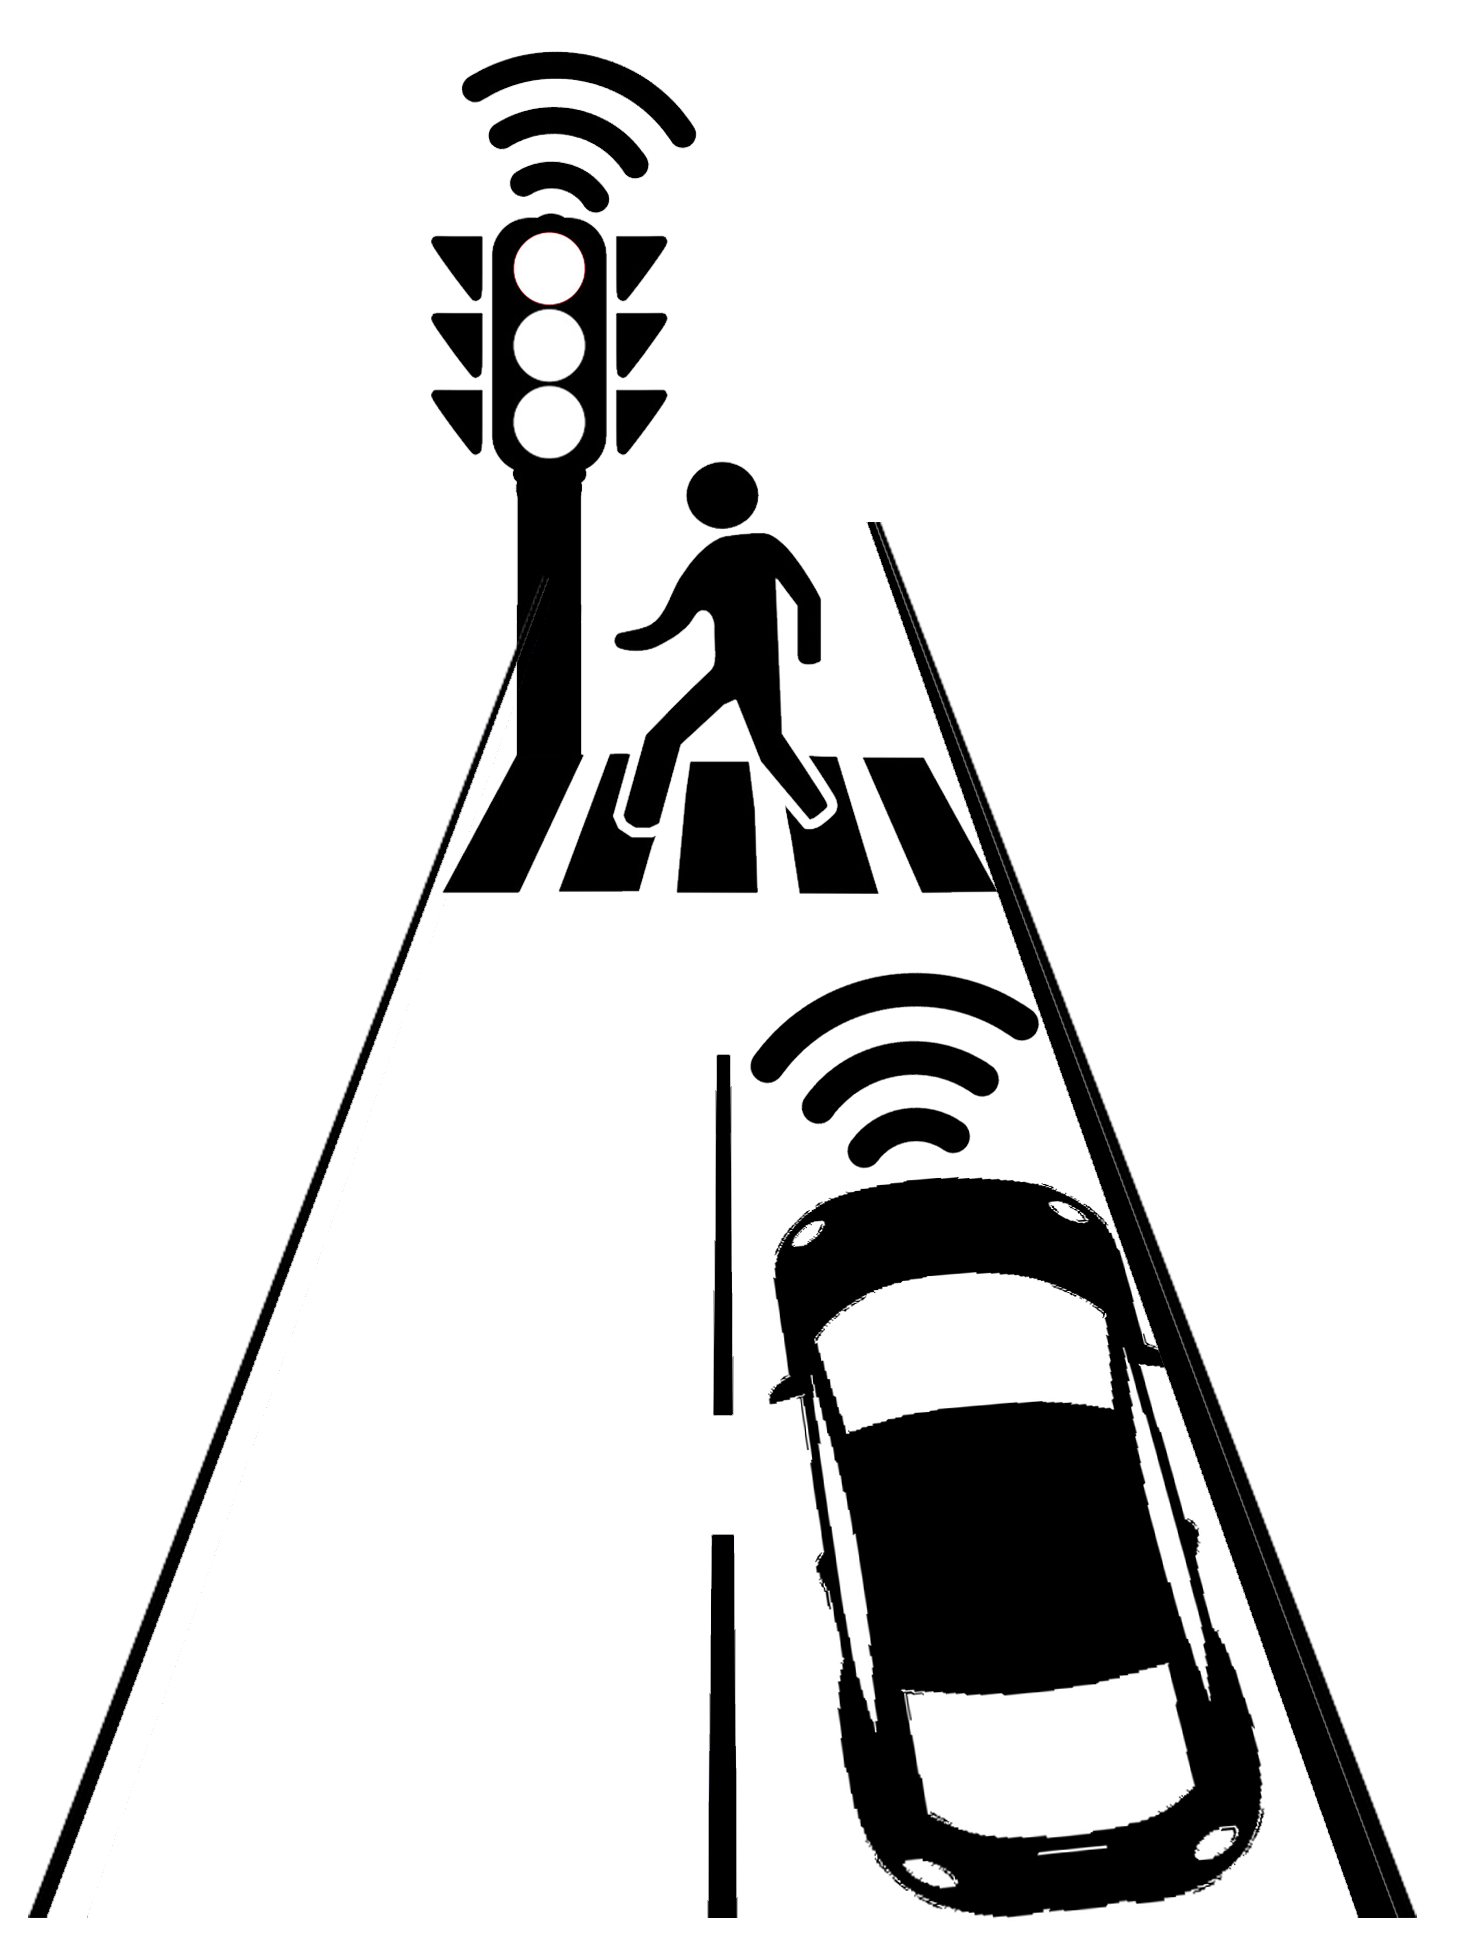
\includegraphics[scale=0.45]{images/V2I.png}
    \caption{Example on V2I}
\end{figure}

\paragraph{}
V2X communication means that vehicles exchange information with each
other and the nearby infrastructure. This new concept is associated with Intelligent Transportation Systems (ITS), a technology with the aim to reduce traffic jam, the environmental impact of transportation and most importantly, to reduce lethal traffic accidents. To enable this technology, wireless communication is needed. Therefore a system that communicates with cars, infrastructure or other vehicles to lower the percentage of fatal accidents is very sought-after. Vehicle manufacturers have been developing this technology for a long time but right now they are facing problems with latency. The existing system depends on a cloud service which has too high latency and this presents a difficult problem in situations where a microsecond could make a big difference in saving the lives of road travellers.

\newpage
\subsection{Purpose}
The purpose of the project is to make a pilot-study for a future development of "V2X" for Cybercom, therefore we decided to make a simple program that can parse information to a database from a log file. To apply in a real world situation we chose to have a back story, see Figure 1, where a pedestrian has pressed the button on a crosswalk traffic light and is about to cross the street. Our task is to structure a future implementation of the V2I program which warns both the pedestrian and the car that either one of them is approaching/trying to cross a crosswalk.

\subsection{Limitations}
The limitations for this project is that only the basic implementation of V2I will be tested. V2V is already a working concept and won't be altered. There will be no safety checks either. The ambition of the project is to test the implementation of V2I in forms of reading a log file and to compare two positions acquired from the file. It will be limited to parse information from the log file supplied by Cybercom. In the beginning of the project the software OTTO and Oscar - OTTO is a simulation environment and Oscar is a program used to communicate through ITS-G5 - should have been supplied by Cybercom, but due to lack of time and secrecy we chose not to use them.  
